% An agent-operated, market-anchored forecasting system: the 2026 World Cup Probability Cup.
% Build: `make paper` from the repository root (figures, numbers and tables are generated
% from results/data by paper/build_assets.py before LaTeX runs).
\documentclass[11pt]{article}
% Reproducible output: no build dates or random trailer ID, so a rebuild changes no bytes.
\ifdefined\pdfinfoomitdate \pdfinfoomitdate=1 \pdftrailerid{} \pdfsuppressptexinfo=-1 \fi

\usepackage[T1]{fontenc}
\usepackage[utf8]{inputenc}
\usepackage{lmodern}
\usepackage[letterpaper, margin=1in]{geometry}
\usepackage{microtype}
\usepackage{amsmath, amssymb, mathtools}
\usepackage{booktabs, array, tabularx, makecell}
\usepackage{graphicx}
\usepackage[font=small, labelfont=bf, labelsep=period, skip=5pt]{caption}
\usepackage{xcolor}
\usepackage{enumitem}
\usepackage{placeins}
\usepackage{etoolbox}
\usepackage{tikz}
\usetikzlibrary{arrows.meta, positioning, calc, fit, backgrounds}
\usepackage[round, sort&compress]{natbib}
\usepackage{xurl}
\usepackage[colorlinks=true, linkcolor=linkblue, citecolor=linkblue, urlcolor=linkblue,
            pdftitle={An Agent-Operated, Market-Anchored Forecasting System},
            pdfauthor={Yifan Luo},
            pdfkeywords={probabilistic forecasting, Brier score, football, Dixon-Coles,
                         wisdom of crowds, language-model agents}]{hyperref}
\usepackage[capitalise, noabbrev]{cleveref}

\definecolor{linkblue}{HTML}{1F5FAD}
\definecolor{series1}{HTML}{2A78D6}
\definecolor{series2}{HTML}{EB6834}
\definecolor{ink2}{HTML}{52514E}

\setlist{itemsep=2pt, topsep=4pt, parsep=0pt}
\setlength{\tabcolsep}{5pt}
\renewcommand{\arraystretch}{1.1}

\newcommand{\RBP}{\mathrm{RBP}}
\newcommand{\code}[1]{\texttt{\detokenize{#1}}}
\newcommand{\ci}[2]{{\footnotesize\,[#1,\,#2]}}
\newcommand{\nohyphens}{\hyphenpenalty=10000\exhyphenpenalty=10000\relax}
\newcolumntype{L}{>{\raggedright\arraybackslash}X}
\AtBeginEnvironment{table}{\small}
\setlength{\bibsep}{3pt plus 1pt}
\renewcommand{\bibfont}{\small}

% Generated by paper/build_assets.py from results/data — do not edit by hand.
\newcommand{\MarketsOne}{1,183}
\newcommand{\MatchesOne}{103}
\newcommand{\PointsOne}{4,732}
\newcommand{\PointsOneExact}{4,731.9}
\newcommand{\PointsOneLo}{3,299}
\newcommand{\PointsOneHi}{6,342}
\newcommand{\BrierOne}{0.2197}
\newcommand{\ConsensusBrierOne}{0.2206}
\newcommand{\FieldBrierOne}{0.2457}
\newcommand{\AboveFieldOne}{69.1}
\newcommand{\CloserOne}{57.0}
\newcommand{\PremiumOne}{4,275}
\newcommand{\PremiumOneLo}{3,672}
\newcommand{\PremiumOneHi}{4,908}
\newcommand{\PremiumShareOne}{90}
\newcommand{\PremiumPerMarketOne}{3.61}
\newcommand{\EdgeOne}{$+$457}
\newcommand{\EdgeOneLo}{$-$751}
\newcommand{\EdgeOneHi}{$+$1,754}
\newcommand{\EdgePerMarketOne}{$+$0.39}
\newcommand{\EdgePerMarketOneLo}{$-$0.63}
\newcommand{\EdgePerMarketOneHi}{$+$1.47}
\newcommand{\GroupPointsOne}{1,593}
\newcommand{\GroupMarketsOne}{699}
\newcommand{\KnockoutPointsOne}{2,637}
\newcommand{\KnockoutMarketsOne}{464}
\newcommand{\FinalPointsOne}{501.6}
\newcommand{\AfterGroupShareOne}{66}
\newcommand{\MarketsTwo}{1,035}
\newcommand{\MatchesTwo}{88}
\newcommand{\PointsTwo}{4,451}
\newcommand{\PointsTwoExact}{4,451.1}
\newcommand{\PointsTwoLo}{3,072}
\newcommand{\PointsTwoHi}{6,020}
\newcommand{\BrierTwo}{0.2174}
\newcommand{\ConsensusBrierTwo}{0.2194}
\newcommand{\FieldBrierTwo}{0.2437}
\newcommand{\AboveFieldTwo}{69.7}
\newcommand{\CloserTwo}{57.3}
\newcommand{\PremiumTwo}{3,820}
\newcommand{\PremiumTwoLo}{3,259}
\newcommand{\PremiumTwoHi}{4,475}
\newcommand{\PremiumShareTwo}{86}
\newcommand{\PremiumPerMarketTwo}{3.69}
\newcommand{\EdgeTwo}{$+$631}
\newcommand{\EdgeTwoLo}{$-$527}
\newcommand{\EdgeTwoHi}{$+$1,846}
\newcommand{\EdgePerMarketTwo}{$+$0.61}
\newcommand{\EdgePerMarketTwoLo}{$-$0.52}
\newcommand{\EdgePerMarketTwoHi}{$+$1.75}
\newcommand{\GroupPointsTwo}{1,169}
\newcommand{\GroupMarketsTwo}{551}
\newcommand{\KnockoutPointsTwo}{2,781}
\newcommand{\KnockoutMarketsTwo}{464}
\newcommand{\FinalPointsTwo}{501.6}
\newcommand{\AfterGroupShareTwo}{74}
\newcommand{\MarketsBoth}{2,218}
\newcommand{\FieldSD}{16}
\newcommand{\FieldVariance}{0.0251}
\newcommand{\GroupMatches}{71}
\newcommand{\KnockoutMatches}{32}
\newcommand{\ECEOurs}{0.030}
\newcommand{\ECECrowd}{0.057}
\newcommand{\RELOurs}{0.0018}
\newcommand{\RELCrowd}{0.0051}
\newcommand{\RESOurs}{0.0239}
\newcommand{\RESCrowd}{0.0283}
\newcommand{\UNC}{0.2439}
\newcommand{\MeanForecast}{42.2}
\newcommand{\MeanCrowd}{47.1}
\newcommand{\BaseRate}{42.2}
\newcommand{\CommonMarkets}{1,035}
\newcommand{\DivergentMarkets}{112}
\newcommand{\DivergentMatches}{36}
\newcommand{\BotTwoBetter}{59}
\newcommand{\BotOneBetter}{53}
\newcommand{\ABNet}{$+$93.7}
\newcommand{\ABLo}{$-$215}
\newcommand{\ABHi}{$+$421}
\newcommand{\CommonBrierOne}{0.2176}
\newcommand{\CommonBrierTwo}{0.2174}
\newcommand{\BotOneOnlyMarkets}{148}
\newcommand{\BotOneOnlyMatches}{15}
\newcommand{\BotOneOnlyPoints}{374.5}
\newcommand{\BotTwoFirstMatch}{16}
\newcommand{\GapPoints}{280.8}
\newcommand{\CrowdBiasCards}{$+$13.3}
\newcommand{\OurBiasCards}{$+$6.6}
\newcommand{\OurBiasAbsCards}{6.6}
\newcommand{\EdgeCards}{$+$155}
\newcommand{\EdgePerMarketCards}{$+$1.7}
\newcommand{\MarketsCards}{90}
\newcommand{\CrowdBiasPlayerSOT}{$+$12.4}
\newcommand{\OurBiasPlayerSOT}{$+$0.4}
\newcommand{\OurBiasAbsPlayerSOT}{0.4}
\newcommand{\EdgePlayerSOT}{$+$122}
\newcommand{\EdgePerMarketPlayerSOT}{$+$1.1}
\newcommand{\MarketsPlayerSOT}{116}
\newcommand{\CrowdBiasPenalties}{$+$10.9}
\newcommand{\OurBiasPenalties}{$+$11.3}
\newcommand{\OurBiasAbsPenalties}{11.3}
\newcommand{\EdgePenalties}{$+$33}
\newcommand{\EdgePerMarketPenalties}{$+$0.6}
\newcommand{\MarketsPenalties}{55}
\newcommand{\CrowdBiasScorers}{$+$10.5}
\newcommand{\OurBiasScorers}{$+$4.7}
\newcommand{\OurBiasAbsScorers}{4.7}
\newcommand{\EdgeScorers}{$+$40}
\newcommand{\EdgePerMarketScorers}{$+$0.3}
\newcommand{\MarketsScorers}{121}
\newcommand{\CrowdBiasTiming}{$+$7.3}
\newcommand{\OurBiasTiming}{$+$5.0}
\newcommand{\OurBiasAbsTiming}{5.0}
\newcommand{\EdgeTiming}{$+$85}
\newcommand{\EdgePerMarketTiming}{$+$2.9}
\newcommand{\MarketsTiming}{29}
\newcommand{\CrowdBiasGoals}{$-$0.8}
\newcommand{\OurBiasGoals}{$-$2.1}
\newcommand{\OurBiasAbsGoals}{2.1}
\newcommand{\EdgeGoals}{$+$279}
\newcommand{\EdgePerMarketGoals}{$+$0.7}
\newcommand{\MarketsGoals}{379}
\newcommand{\CrowdBiasTeamSOT}{$+$3.5}
\newcommand{\OurBiasTeamSOT}{$-$5.7}
\newcommand{\OurBiasAbsTeamSOT}{5.7}
\newcommand{\EdgeTeamSOT}{$-$215}
\newcommand{\EdgePerMarketTeamSOT}{$-$1.4}
\newcommand{\MarketsTeamSOT}{158}
\newcommand{\DevPointsLowest}{$+$6.5}
\newcommand{\DevPointsNear}{$+$3.5}
\newcommand{\DevPointsHighest}{$-$2.0}
\newcommand{\BelowMarkets}{506}
\newcommand{\AboveMarkets}{119}
\newcommand{\FarAboveMarkets}{18}
\newcommand{\NearMarkets}{558}
\newcommand{\BacktestForecasts}{782,157}
\newcommand{\BacktestFamilies}{19}
\newcommand{\BacktestBeatHalf}{19}
\newcommand{\BacktestBeatBase}{17}
\newcommand{\BacktestPerFamily}{41,163}
\newcommand{\RunsTotal}{254}
\newcommand{\RunsSubmit}{201}
\newcommand{\RunsPreview}{53}
\newcommand{\ActionsTotal}{17,005}
\newcommand{\ActionsCreate}{2,158}
\newcommand{\ActionsUpdate}{3,986}
\newcommand{\ActionsUnchanged}{10,711}
\newcommand{\ActionsError}{149}
\newcommand{\OperatedDays}{38}
\newcommand{\Boards}{101}
\newcommand{\BoardMarkets}{1,153}
\newcommand{\numfamilies}{65}

% Generated table bodies go through the TeX primitive, which (unlike \input) is
% expandable inside a tabular, so \bottomrule can follow the last row.
\makeatletter\newcommand*{\inputtable}[1]{\@@input #1 }\makeatother

\title{\textbf{An Agent-Operated, Market-Anchored}\\\textbf{Forecasting System}\\[8pt]
       \Large Lessons from the 2026 World Cup Probability Cup}
\author{Yifan Luo\\[3pt]
        \normalsize Code and data: \url{https://github.com/im-yifanluo/jump-probability-cup}}
\date{Technical report, October 2026}

\begin{document}
\maketitle

\begin{abstract}
\noindent
The Jump Trading Probability Cup asked forecasters for probabilities on about ten binary
questions per match of the 2026 FIFA World Cup and ranked 4,013 entries by Brier score relative
to the field. This report describes the system behind two of those entries and the agent that
operated it. The forecasting engine never rates teams itself: it fits a Dixon--Coles scoreline
distribution to de-margined bookmaker and prediction-market odds and derives everything else
from it---corners, cards, shots and offsides through negative-binomial models regressed on
odds-implied scoring rates in about 41,000 club matches, and player props from confirmed
lineups---so that answers across \numfamilies{} question families are mutually consistent. For
\OperatedDays{} days a Claude Code agent ran the system in production: it scheduled its own
pre-kickoff passes, researched inputs the market misses, submitted and verified both entries,
and ran a live A/B test on the second entry under a fixed promotion rule. The stable entry
finished 17th overall and the experimental entry 5th in the knockout stage. The relative score
decomposes exactly into an \emph{edge} over the crowd's average forecast and a \emph{premium}
equal to the dispersion of the field's forecasts. The premium accounts for \PremiumShareOne\%
of the stable entry's points; the edge is positive for both entries and concentrated where the
crowd over-prices rare events, but it is not distinguishable from zero over \MatchesOne{}
matches. We also report the operating incidents that shaped the system's guardrails and a
differential-testing harness that pins the archived code to its tournament behaviour.
\end{abstract}

\noindent\textbf{Keywords:} probabilistic forecasting, Brier score, association football,
Dixon--Coles, wisdom of crowds, language-model agents, ML operations

% ---------------------------------------------------------------------------
\section{Introduction}\label{sec:intro}

Forecasting tournaments reward probabilities that are both calibrated and sharp, and the best
human forecasters in them combine careful base rates with fast updating on new information
\citep{mellers2014, tetlock2015}. In June 2026 Jump Trading sponsored such a tournament for the
FIFA World Cup: the Probability Cup, hosted on SportsPredict and run as a recruiting contest
\citep{jump2026}. Each of the tournament's 104 matches carried about ten yes/no
questions---from ``Will Argentina win?'' to ``Will a goal be scored before the first hydration
break?''---each answered with a whole-number probability before kickoff and scored by its Brier
score relative to the field \citep{sportspredict2026}. Bots were allowed, two per person, each
ranked as its own entry.

The problem is hard in three specific ways. The questions are \emph{broad}: they span goals,
halves, timing windows, corners, cards, shots, offsides, fouls, scorers, player shots on
target, substitutions and advancement, and most have no betting market. The information is
\emph{late}: starting lineups appear about an hour before kickoff, the deadline is the
kickoff, and kickoff times change from day to day. And the score is \emph{relative}: each
forecast is compared with the average of thousands of participants, many of whom read the same
public odds.

Our response was to anchor every answer on the betting market, model only what the market does
not price, and treat operating the system as an engineering problem delegated to an agent with
strict guardrails. The contributions are:
\begin{enumerate}[leftmargin=*]
  \item A market-anchored pricing engine that answers \numfamilies{} question families from one
        odds-fitted scoreline grid plus count and player models, so the answers cannot
        contradict each other (\cref{sec:engine}).
  \item An operating design in which a language-model coding agent runs the production loop
        (scheduling, research, submission, verification and experimentation) while every
        submitted number comes out of the statistical pipeline (\cref{sec:ops}).
  \item An exact decomposition of relative Brier scoring into an edge over the crowd's average
        forecast and a premium for the field's dispersion, and an analysis of where the points
        came from (\cref{sec:method,sec:results}).
  \item A record of the incidents that shaped the operating rules (\cref{sec:incidents}) and a
        differential-testing harness that keeps the archived system reproducible
        (\cref{sec:repro}).
\end{enumerate}
The stable entry (bot~1) finished \#17 of 4,013 overall and \#8 in the knockout stage; the
experimental entry (bot~2) finished \#31 overall and \#5 in the knockout stage. On the markets
they played, their mean Brier scores were \BrierOne{} and \BrierTwo{}, against \FieldBrierOne{}
for the average participant on bot~1's markets.

% ---------------------------------------------------------------------------
\section{Background}\label{sec:background}

\paragraph{Scoring.}
For a market $m$ with outcome $y_m\in\{0,1\}$ and stage weight $w_m$ (1 in the group stage,
2 in the knockout rounds, 3 in the final), let $F_m$ be the participants who forecast it,
$q_{im}\in\{0.01,\dots,0.99\}$ their forecasts and
$\bar B_m = |F_m|^{-1}\sum_{i\in F_m}(q_{im}-y_m)^2$ the field-average Brier score
\citep{brier1950}. A forecast $p$ earns \emph{relative Brier points}
\begin{equation}\label{eq:rbp}
  \RBP_m(p) = 100\,w_m\bigl(\bar B_m - (p-y_m)^2\bigr),
\end{equation}
and the leaderboard ranks the sum over all settled markets. Three consequences shaped the
system. First, $\bar B_m$ does not depend on $p$, so the expected score is maximized by
minimizing one's own expected Brier score; because the Brier score is strictly proper, the
optimal report is one's true probability \citep{gneiting2007}, and shading toward or away from
the crowd can only lose in expectation. Second, a forfeited market scores zero, while any
forecast at least as good as the crowd's average scores positive in expectation
(\cref{sec:method}), so coverage has value. Third, late rounds weigh up to three times as much.

\paragraph{Football models and betting markets.}
Goal counts are commonly modelled as Poisson \citep{maher1982}, with the low-score dependence
correction of \citet{dixon1997} or a bivariate Poisson \citep{karlis2003}. Betting odds are
strong forecasts \citep{forrest2005, spann2009}; machine-learning models struggle to beat
closing lines \citep{hubacek2019}, and for betting, calibration matters more than accuracy
\citep{walsh2024}. Implied probabilities must first be de-margined, proportionally or with
Shin's model \citep{shin1993, strumbelj2014}; prediction markets offer a second, independent
price \citep{wolfers2004}. Overdispersed counts such as corners and cards are naturally
negative binomial \citep{cameron2013}.

\paragraph{Crowds.}
The average of many forecasts is usually better than the average forecaster \citep{galton1907}.
For squared error this is an identity: the crowd's error equals the average individual error
minus the diversity of the forecasts \citep{krogh1995, page2007}. It drives our decomposition in
\cref{sec:method}. Aggregates of independent forecasters often benefit from extremizing
\citep{baron2014, satopaa2014}; we tested extremizing for our single, already market-anchored
forecast and rejected it.

\paragraph{Agents and AI forecasting.}
Language-model agents that interleave reasoning and tool use \citep{yao2023} now operate
software environments directly \citep{yang2024}. Language models have also been evaluated as
forecasters, in retrieval-augmented systems \citep{halawi2024}, live tournaments
\citep{schoenegger2023} and dynamic benchmarks \citep{karger2025}; the Probability Cup itself
entered three language models as benchmark bots. Our agent, Claude Code \citep{claudecode}, has
a different role: it does not forecast, but operates a statistical system. That makes the work
an instance of the production-ML concerns raised by \citet{sculley2015}, with an online
controlled experiment \citep{kohavi2020} on the second entry, and with differential testing
\citep{mckeeman1998} and characterization tests \citep{feathers2004} to archive it.

% ---------------------------------------------------------------------------
\section{The forecasting engine}\label{sec:engine}

\Cref{fig:architecture} shows the pipeline. Its organizing rule is a pricing hierarchy: (1)~a
market price for this exact fixture wins where one exists; (2)~otherwise, the output of models
fitted to that price; (3)~otherwise, conditional tables measured on international-tournament
event data \citep{statsbomb}; (4)~only then a base rate, which is always flagged.

\begin{figure}[tbp]
\centering
\begin{tikzpicture}[
    font=\footnotesize, >={Stealth[length=1.6mm]},
    box/.style={draw=black!45, rounded corners=2pt, align=center, inner sep=3pt,
                minimum height=9.5mm, fill=white, line width=0.4pt,
                execute at begin node=\nohyphens},
    data/.style={box, fill=black!5, text width=27mm},
    model/.style={box, fill=series1!8, draw=series1!70!black, text width=24mm},
    botbox/.style={box, text width=21mm},
    agent/.style={box, fill=series2!10, draw=series2!80!black, minimum height=7mm},
    arr/.style={->, black!55, line width=0.45pt},
    agentarr/.style={->, series2!80!black, line width=0.45pt, rounded corners=2pt},
    lab/.style={font=\scriptsize, text=ink2, fill=white, inner sep=1pt}]
  % inputs (column 1) and models (column 2), one row each
  \node[data]  (q)   at (1.55, 0)    {SportsPredict API\\[-1pt]\scriptsize questions, deadlines};
  \node[data]  (o)   at (1.55, -1.4) {Odds feeds\\[-1pt]\scriptsize DraftKings (ESPN),\\[-2pt]\scriptsize Polymarket};
  \node[data]  (tab) at (1.55, -2.8) {Fitted tables\\[-1pt]\scriptsize club count models,\\[-2pt]\scriptsize StatsBomb};
  \node[data]  (in)  at (1.55, -4.2) {Researched inputs\\[-1pt]\scriptsize lineups, referees,\\[-2pt]\scriptsize scorer odds};
  \node[model] (p)   at (5.05, 0)    {Question parser\\[-1pt]\scriptsize \numfamilies{} families};
  \node[model] (g)   at (5.05, -1.4) {Goal grid\\[-1pt]\scriptsize Dixon--Coles fit to odds};
  \node[model] (c)   at (5.05, -2.8) {Count models\\[-1pt]\scriptsize negative binomial};
  \node[model] (pl)  at (5.05, -4.2) {Player models\\[-1pt]\scriptsize scorers,\\[-2pt]\scriptsize shots on target};
  % pricer, bot passes, constants, submission
  \node[model, text width=19mm, minimum height=51mm] (mp) at (8.35, -2.1)
       {MatchPricer\\[2pt]\scriptsize family $\to$ method;\\\scriptsize blend toward\\\scriptsize a baseline};
  \node[botbox] (b2) at (11.4, -1.4) {Bot 2 pass\\[-1pt]\scriptsize experiment constants};
  \node[botbox] (b1) at (11.4, -2.8) {Bot 1 pass\\[-1pt]\scriptsize stable constants};
  \node[data, text width=21mm] (k) at (11.4, -4.2) {Calibration\\[-1pt]\scriptsize constants};
  \node[box, text width=20mm, minimum height=23.5mm] (sub) at (14.55, -2.1)
       {Submit bot 2,\\then bot 1\\[4pt]\scriptsize verify both\\[-2pt]\scriptsize on the platform};
  \node[agent, text width=148mm] (a) at (8.05, 1.45)
       {\textbf{Claude Code agent}: schedules its own runs, researches inputs, runs the pipeline,
        verifies submissions, scores the A/B test and promotes by rule};
  % data flow
  \draw[arr] (q) -- (p);
  \draw[arr] (o) -- (g);
  \draw[arr] (tab) -- (c);
  \draw[arr] (in) -- (pl);
  \draw[arr] ($(in.east)+(0,0.22)$) -- ($(c.west)+(0,-0.22)$);
  \draw[arr] (g) -- (c);
  \draw[arr] (c) -- (pl);
  \foreach \n in {p, g, c, pl} \draw[arr] (\n.east) -- (mp.west |- \n.east);
  \draw[arr] (mp.east |- b2.west) -- (b2.west);
  \draw[arr] (mp.east |- b1.west) -- (b1.west);
  \draw[arr] (k.west) -- (mp.east |- k.west);
  \draw[arr] (b2.east) -- (sub.west |- b2.east);
  \draw[arr] (b1.east) -- (sub.west |- b1.east);
  % the agent's touch points
  \draw[agentarr] (a.west) -| (-0.25, -4.2) -- (in.west)
       node[lab, pos=0.3, rotate=90] {researches};
  \draw[agentarr] (a.south -| mp.north) -- (mp.north) node[lab, midway] {runs};
  \draw[agentarr] (a.south -| sub.north) -- (sub.north) node[lab, midway] {verifies};
  \draw[agentarr] (a.east) -| (16.2, -4.2) -- (k.east) node[lab, pos=0.75] {promotes};
\end{tikzpicture}
\caption{The pipeline. The agent (orange) feeds structured inputs and operates the pipeline; it
never edits the models' output. Both bots are priced from identical odds and inputs; bot~2
reprices under its experiment constants and is submitted first, so bot~1's stable values are
always the last write.}
\label{fig:architecture}
\end{figure}

\subsection{Anchoring on the market}\label{sec:anchor}

For each fixture we take the 1X2 (home, draw, away) prices and the over/under line from the
ESPN feed of DraftKings odds and remove the margin proportionally,
$\pi_k=(1/o_k)/\sum_j(1/o_j)$ \citep{strumbelj2014}. Where Polymarket lists the match, its
de-margined 1X2 is averaged in, and disagreements above 10 points are flagged as likely stale.
The total expected goals $T$ solves $\Pr(N\ge L+\tfrac12)=\pi_{\text{over}}$ for
$N\sim\mathrm{Poisson}(T)$ and line $L$. A dated manual override exists for fixtures without a
feed; it expires loudly on any other date.

\subsection{The goal grid}\label{sec:grid}

Home and away goals $(X,Y)$ follow independent Poisson laws with the Dixon--Coles correction
\citep{dixon1997},
\begin{equation}\label{eq:dc}
  \Pr(X=x,Y=y)\propto\tau(x,y)\,\frac{\lambda_H^{x}e^{-\lambda_H}}{x!}\,
  \frac{\lambda_A^{y}e^{-\lambda_A}}{y!},
\end{equation}
with $\tau(0,0)=1-\lambda_H\lambda_A\rho$, $\tau(1,0)=1+\lambda_A\rho$,
$\tau(0,1)=1+\lambda_H\rho$, $\tau(1,1)=1-\rho$ and $\tau=1$ elsewhere, on a grid truncated at
12 goals and renormalized. The parameters are not estimated from team histories. With
$\lambda_A=T-\lambda_H$, we solve for $(\lambda_H,\rho)$ such that the grid reproduces the
market's home-win and draw probabilities exactly, with $\rho$ clamped to keep every cell
non-negative. Every goal question is then a sum over cells of one grid: results, totals, both
teams scoring, margins, clean sheets and combinations (``both teams score and 3+ goals'' is a
joint sum, never a product of marginals). Half-based questions split each rate into halves with
the second-half share $h=0.60$ measured on international tournaments (club football gives
0.54). The first goal is a Poisson race, $\Pr(\text{team scores first})=
\lambda_{\text{team}}/(\lambda_H+\lambda_A)\cdot(1-\Pr(0,0))$; a large-sample check on 219
tournament matches confirmed that goals are exchangeable in time (observed 0.886, model 0.878).
Advancement in a knockout tie adds extra time and penalties explicitly:
\begin{equation}\label{eq:advance}
  \Pr(A\text{ advances})=\Pr(X_A>X_B)+\Pr(X_A=X_B)\bigl[\Pr(E_A>E_B)+\Pr(E_A=E_B)\,s\bigr],
\end{equation}
where $E_A,E_B$ are Poisson extra-time goals at a third of each side's 90-minute rate and the
shoot-out share $s=\tfrac12+\kappa(\sigma_A-\tfrac12)$ shrinks the regulation strength share
$\sigma_A=\Pr(X_A>X_B)/(\Pr(X_A>X_B)+\Pr(X_A<X_B))$ toward a coin flip ($\kappa=0.25$). The two
sides' probabilities sum to one exactly, and the shoot-out market uses the same extra-time
Poissons.

\subsection{Count models}\label{sec:counts}

Corners, cards, shots on target (SOT) and fouls use negative-binomial (NB2) models fitted on
club football from football-data.co.uk \citep{footballdata}: the 40,596 matches before the
2025/26 season (out of 115,987 in 19 leagues) that have both match statistics and closing 1X2
and over/under odds. The odds give each match the same odds-implied rates
$(\lambda_{\text{team}},\lambda_{\text{opp}})$ that the live system computes:
\begin{equation}\label{eq:counts}
  \log\mu_k=\beta_{0k}+\beta_{1k}\log\lambda_{\text{team}}+\beta_{2k}\log\lambda_{\text{opp}}
  +\beta_{3k}\,\text{home},\qquad\operatorname{Var}=\mu_k(1+\alpha_k\mu_k).
\end{equation}
The coefficients come from a Poisson GLM and $\alpha_k$ from the moment estimator of
\citet{cameron2013} (\cref{tab:counts}). Because the covariates are market-implied rather than
team identities, the fit transfers to any fixture with odds. At the World Cup the venue is
neutral (home $=\tfrac12$) and each mean is multiplied by tournament corrections (below) and, for
cards, by the referee's strictness, $(\text{referee cards per game})/3.46$, capped at~1.
Totals are exact convolutions of the two team distributions (a sum of unequal-mean NBs is not
NB), and ``more X than'' comparisons enumerate both, with ties resolving to No. Offsides have
no club coverage and depend more on defensive lines than on attacking strength: their mean is
the tournament team mean times $(\lambda_{\text{team}}/1.30)^{0.18}$, an elasticity measured on
event data. Timing-window questions (``a goal before the first hydration break'') use the share
of each event type falling in that window, measured from event timestamps, applied to the
match mean.

\begin{table}[tbp]
\centering
\caption{Count models fitted on club matches (\cref{eq:counts}). Shots on target scale almost
proportionally with a team's own odds-implied scoring rate; cards and fouls fall as a team gets
stronger.}
\label{tab:counts}
\begin{tabular}{lrrrrr}
\toprule
Statistic & $\beta_0$ & $\beta_1$ (own rate) & $\beta_2$ (opponent) & $\beta_3$ (home) & $\alpha$ \\
\midrule
\inputtable{generated/tab_count_models.tex}
\bottomrule
\end{tabular}
\end{table}

\subsection{Players}\label{sec:players}

A player's anytime-scorer probability is $1-\exp(-g\,\lambda_{\text{team}}\,m/90)$, where $g$
is the player's share of team goals, shrunk toward 0.12 with a prior weight of six team goals, and
$m$ is the player's expected minutes. Minutes come from the confirmed starting XI, which the
pipeline pulls from ESPN as soon as it is posted; a benched player's minutes drop
automatically. Shots on target use a per-match rate $r$: a club rate times 0.839 (tournament
play is less open), shrunk toward 0.72 with the weight of one appearance, then multiplied by
the match tempo $\min(\mu^{\text{SOT}}_{\text{team}}/4.11,\,1.6)$ and by $m/90$. For the
threshold of one SOT and a genuine shooter ($r\ge0.5$) the tempo swing is halved, because a
starter shoots regardless of the opponent; this lowered held-out Brier from 0.275 to 0.255 on
234 shooter-matches. A leave-one-tournament-out check of the SOT model on 4,989 player-matches
gave a Brier score of 0.174, against 0.212 for the previous model and 0.250 for a coin flip.

Scorer markets are the one place where a researched number replaces the model: a de-margined
anytime-scorer price for this exact fixture, $p=(1/o)/1.10$, tagged with the fixture name and
expiring loudly if reused for another match. For a star confirmed on the bench, the agent
prices the cameo explicitly, as the probability of coming on times the probability of scoring
in the expected minutes. Score-or-assist markets are kept consistent with these anchors by a
sweep: each must sit at or above the anytime price plus an assist uplift.

\subsection{Tuned constants and coverage}\label{sec:constants}

Every tuned constant lives in one module, which the models read at call time; that is what
lets bot~2 reprice under different constants (\cref{sec:ab}). \Cref{tab:constants} lists the
corrections that ran in the final. They are multiplicative and \emph{level-specific}: a
per-team scale also moves totals, but a total-only scale never touches per-team or
comparison markets, which are scale-invariant. An early uniform ``low-event'' multiplier on every
count statistic dropped bot~1 from about 50th to 94th within days; per-statistic corrections,
validated out of sample, replaced it. Families whose models showed weak out-of-sample skill are
shrunk toward the same machinery run at tournament-average rates,
$p=p_{\text{base}}+w\,(p_{\text{model}}-p_{\text{base}})$, with weights from the club backtest
(0.40 for card thresholds, 0.67 for ``more goals in the second half'').

\begin{table}[tbp]
\centering
\caption{The tournament corrections that ran in the final (all in \code{models/calibration.py}).}
\label{tab:constants}
\begin{tabularx}{\textwidth}{@{}l >{\raggedright\arraybackslash}p{30mm} l L@{}}
\toprule
Constant & Value & Scope & Evidence \\
\midrule
Tournament intensity & cards 0.78, SOT 1.00, corners 1.05, offsides and fouls 0.90
  & per-team means & Re-fitted per statistic on 383 settled markets with chronological
  out-of-sample validation, replacing a uniform 0.90 \\
Total SOT scale & 1.50 & totals only & The platform counts about 1.5$\times$ the event-data total
  (implied 1.49, 95\% CI 1.24--1.78); bot-2 probe won 4 of 5 \\
Total cards scale & 0.85 & totals only & Cards over-predicted by 0.05 on 724 markets; bot-2 probe
  won 8 of 13 \\
Total offsides scale & 1.10 & totals only & Consistent under-prediction of totals \\
Favourite SOT boost & 0.06 & favourite only & Club elasticity too flat for mismatches; probe won
  4 of 4 divergent markets \\
Timing scale & 0.85 & timing windows & Realized 0.214 vs 0.432 priced ($n=28$); probe 5 of 6;
  walk-forward $-1.83$ Brier points \\
Referee factor & $\le 1$ & cards & Strict referees over-predicted cards; only leniency is priced \\
Shoot-out tilt $\kappa$ & 0.25 & advancement & Shoot-outs are close to coin flips \\
\bottomrule
\end{tabularx}
\end{table}

Questions arrive as free text. About a hundred small rules map each to a structured
specification (family, team, player, statistic, threshold, period); all \BoardMarkets{}
questions on the \Boards{} archived boards parse into \numfamilies{} families
(\cref{tab:families}). Anything unrecognized is logged and never priced by guesswork. When the
knockout boards re-phrased every question with ``in regulation (90 minutes + stoppage time)'',
a normalizer let the group-stage rules serve them, and 19 new families were built and tested
during the knockouts, each on the day it appeared.

% ---------------------------------------------------------------------------
\section{Operating the system with an agent}\label{sec:ops}

\Cref{tab:roles} divides the work. The statistical pipeline produces every probability. The
agent, a Claude Code session working from three checklist playbooks, does everything around
it, and the operator (the author) sets objectives and rules.

\begin{table}[tbp]
\centering
\caption{Division of labour.}
\label{tab:roles}
\begin{tabularx}{\textwidth}{@{}l L@{}}
\toprule
Role & Responsibility \\
\midrule
Pipeline & Every probability: odds-anchored goal grid, count and player models, one pricer per match. \\
Agent & Inputs the market misses (confirmed lineups, referee strictness, de-margined scorer prices),
  written to match-scoped files; running the pipeline on schedule; verifying submissions;
  running and scoring the A/B bench; reports and long-term memory notes. \\
Operator & Objectives and rules: standing authorization for bot-1 submissions (June~12) and for
  promoting validated probes (July~2); quality over coverage; the final-day objectives. \\
\bottomrule
\end{tabularx}
\end{table}

\subsection{The daily cycle}\label{sec:cycle}

Kickoff times moved every day, so fixed-time runs kept missing the short window between the
lineup release (about 60 minutes before kickoff) and the deadline (kickoff). The agent therefore
scheduled its own day (\cref{fig:day}). A morning run scored the previous day's markets,
scored the A/B probes, researched the day's matches, submitted both bots for the next 48 hours,
verified them and printed one-shot schedule entries for 50 minutes before each kickoff wave. Each
pass then pulled the confirmed lineups, the final odds and the referee and resubmitted; the last
pass of the day also priced the next day. A late pass costs freshness, never correctness: the
pipeline refuses to write to a market whose kickoff has passed.

\begin{figure}[tbp]
\centering
\begin{tikzpicture}[x=0.92cm, y=1cm, font=\footnotesize, >={Stealth[length=1.5mm]}]
  % hours
  \draw[black!45, line width=0.5pt] (7,0) -- (23.4,0);
  \foreach \h in {8,10,...,22}
    \draw[black!45] (\h,0) -- (\h,-0.08) node[below=1pt, font=\scriptsize, text=ink2] {\h:00};
  % watchdog: an OS cron every 20 minutes, alerts only
  \foreach \t in {7.333,7.667,...,23.3}
    \fill[black!30] (\t,-0.72) circle (0.6pt);
  \node[anchor=east, font=\scriptsize, text=ink2] at (7.2,-0.72) {watchdog};
  \node[anchor=north east, font=\scriptsize, text=ink2] at (23.4,-0.86)
       {OS cron every 20 min: raises an alarm if a run is missing, never submits};
  % morning run
  \node[draw=series2!80!black, fill=series2!10, rounded corners=2pt, align=left,
        anchor=south west, inner sep=3pt] (m) at (7.45,2.05)
       {\textbf{Morning run}, 07:48: score yesterday and the A/B probes, research today's
        matches,\\ submit both bots for 48 hours, verify, schedule today's passes};
  \draw[series2!80!black, line width=0.5pt, ->] (7.8,2.05) -- (7.8,0.05);
  % kickoff waves: lineups (XI) about 60 min before, a final pass 50 min before
  \foreach \k [count=\i] in {11,14,17,20} {
    \fill[black] (\k,0) circle (1.7pt);
    \node[font=\scriptsize, text=ink2, above=1pt] at (\k,0.04) {kickoff};
    \draw[black!45] (\k-1,0) -- (\k-1,0.16);
    \node[font=\scriptsize, text=ink2, anchor=south east, inner sep=1pt] at (\k-1.02,0.1) {XI};
    \draw[series1!80!black, line width=0.5pt, ->] (\k-0.833,0.98) -- (\k-0.833,0.05);
    \node[draw=series1!70!black, fill=series1!8, rounded corners=2pt, align=center,
          anchor=south, inner sep=2pt, font=\scriptsize] at (\k-0.833,0.98)
         {\ifnum\i=4 last pass,\\+ tomorrow\else final pass,\\$-$50 min\fi};
  }
\end{tikzpicture}
\caption{An illustrative match day with four kickoff waves (local time). The morning run
schedules one final pass 50 minutes before each wave, just after the confirmed lineups (XI)
appear; the last pass also prices the next day. A durable operating-system job checks every
20 minutes that each scheduled run happened and raises an alarm if not.}
\label{fig:day}
\end{figure}

\subsection{Guardrails}\label{sec:guardrails}

\begin{itemize}[leftmargin=*]
  \item \textbf{Inputs, not numbers.} Research enters only through structured files, each entry
        scoped to one match; an input reused for another fixture expires loudly.
  \item \textbf{Contamination-safe order.} Both bots are priced from the same odds; bot~2 is
        submitted first and bot~1 last, so the stable values are always the final write.
  \item \textbf{Verify, don't trust the summary.} After every pass the agent queries both entries
        on the platform and compares their open-prediction counts.
  \item \textbf{Quality over coverage.} No mechanical fallback ever submits. A skipped refresh
        costs only freshness, because the previous submission stands; a careless one can cost
        points. A missed run raises an alarm and a researched run is triggered.
  \item \textbf{Memory outside the context window.} Sessions restart, so decisions, root causes
        and constants were kept in 21 short notes indexed in a file that loads at the start of
        every session, alongside the playbooks, the strategy document and the logs.
\end{itemize}

\subsection{The A/B bench}\label{sec:ab}

Bot~2 tested one family of changes at a time against bot~1's configuration. A context manager
swaps any of eight calibration constants for one pricing pass and always restores them, so both
bots see identical odds and inputs and the strategy is the only difference. A probe was
promoted to bot~1 after it won about 8--10 of its own settled markets in a consistent
direction, counting only markets settled \emph{after} bot~1's last change to that constant (a
tally that ignored this once credited a probe with 10 wins out of 13 when its clean sample was
empty). Live drift flags were treated as hypotheses for large-sample tests, never as fixes:
three of the four raised in the knockouts (first goal, both teams scoring, knockout tempo) were
cleared on event or club data. \Cref{tab:ab} lists the decisions.

\begin{table}[tbp]
\centering
\caption{Probes run on bot~2 and their outcomes. ``Won $k$ of $n$'' counts settled markets
where the two bots differed.}
\label{tab:ab}
\begin{tabularx}{\textwidth}{@{}>{\raggedright\arraybackslash}p{38mm} l L >{\raggedright\arraybackslash}p{23mm}@{}}
\toprule
Probe & Dates & Evidence & Outcome \\
\midrule
Stronger count multipliers & Jun 26--29 & Trailed bot~1 by about 0.015 Brier on 33 differing markets & Rejected \\
Total SOT scale 1.40 & Jun 29 & Same-day natural experiment; total-SOT leave-out Brier 0.245 $\to$ 0.142 & Promoted (totals only) \\
Total SOT scale 1.60 & Jun 29--Jul 2 & Won 4 of 5 against 1.40; implied scale 1.49 & Bot~1 set to 1.50 \\
Total cards 0.85, offsides 1.10, favourite SOT 0.06 & Jul 1--2 & Won 8 of 13 card settles and 4 of 4 favourite-SOT divergents; calibration corroborated & Promoted \\
Total shots 1.10--1.20 & Jul 1--7 & Net loss & Retired \\
Timing scale 0.85 & Jul 3--10 & Won 5 of 6; calibration gap $+0.146$; walk-forward backtest & Promoted \\
Next notches: cards 0.80, timing 0.70, total SOT 1.60, favourite 0.10, offsides 1.20 & Jul 3--19 & Timing 0.70 lost 5 of 5; cards 0.80 net loss ($n=11$); others flat or negative & Retired \\
\bottomrule
\end{tabularx}
\end{table}

\subsection{Activity}

Over \OperatedDays{} days the agent ran the production pipeline \RunsTotal{} times
(\RunsSubmit{} submitting runs and \RunsPreview{} dry runs) and logged \ActionsTotal{}
submission actions: \ActionsCreate{} creates, \ActionsUpdate{} updates, \ActionsUnchanged{}
checks that left a prediction unchanged and \ActionsError{} errors (\cref{fig:activity}). It
wrote 110 run reports and an experiment log with every verdict.

\begin{figure}[tbp]
\centering
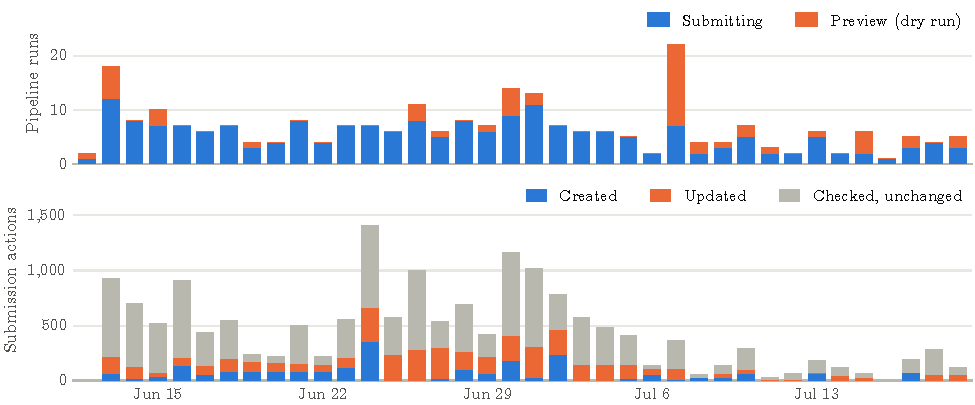
\includegraphics[width=\textwidth]{figures/agent_activity.pdf}
\caption{Daily operation, June 12 to July 19. Top: production-pipeline runs. Bottom: submission
actions across both entries; most were idempotent checks of predictions already in place.}
\label{fig:activity}
\end{figure}

% ---------------------------------------------------------------------------
\section{Evaluation method}\label{sec:method}

\paragraph{Data.}
After the event the platform's results endpoint returned, for every settled market, our
probability, the crowd's average probability $\bar q_m$ (rounded to a whole percent), the
outcome and the stage-weighted points. The export covers \MarketsOne{} markets in \MatchesOne{}
matches for bot~1 and \MarketsTwo{} in \MatchesTwo{} matches for bot~2. Stage weights come from
the question wording (knockout questions carry the regulation qualifier) and the final's match
identifier.

\paragraph{Decomposition.}
For squared error the field-average score splits into the score of the average forecast and the
spread of the forecasts around it \citep{krogh1995, page2007}:
$\bar B_m=(\bar q_m-y_m)^2+V_m$ with $V_m=|F_m|^{-1}\sum_{i\in F_m}(q_{im}-\bar q_m)^2$.
Substituting into \cref{eq:rbp},
\begin{equation}\label{eq:decomp}
  \RBP_m(p)=\underbrace{100\,w_m\bigl[(\bar q_m-y_m)^2-(p-y_m)^2\bigr]}_{\text{edge }E_m}
           +\underbrace{100\,w_m V_m}_{\text{premium }P_m}.
\end{equation}
The premium does not depend on our forecast; every participant who forecasts market $m$
receives it on top of their own edge. Every other term in \cref{eq:decomp} is in the export,
so $V_m$ can be recovered market by market, assuming the platform computes the crowd's average
and the field-average score over the same participants. It must be non-negative, which checks
the stage weights: with the weights above, the recovered $V_m$ is positive on all \MarketsBoth{} markets.
Rounding $\bar q_m$ to a whole percent perturbs each $V_m$ by less than 0.01. The average
recovered $V_m$ is \FieldVariance{}: a typical participant's forecast sits about \FieldSD{}
points from the crowd's average. Note that the premium is not available to any single
forecaster for free: the crowd's average was not visible before kickoff.

\paragraph{Uncertainty.}
Markets within a match settle together (one lopsided match decides a dozen of them), so we
resample whole matches \citep{efron1979, cameron2008}, with 4,000 resamples, and report 95\%
percentile intervals.

\paragraph{Calibration.}
We report reliability diagrams, the expected calibration error over ten equal-width bins
\citep{guo2017} and the corresponding binned Murphy decomposition of the Brier score into
reliability, resolution and uncertainty \citep{murphy1973, degroot1983}.

\paragraph{Offline validation.}
Before the tournament, a walk-forward backtest rebuilt the pricer for every club match with
closing odds in nine test seasons (2017/18 to 2025/26), with count models fitted only on
earlier seasons, and scored \BacktestFamilies{} synthetic question families against what
happened: \BacktestForecasts{} forecasts in all (\cref{tab:backtest}).

% ---------------------------------------------------------------------------
\section{Results}\label{sec:results}

\subsection{Where the points came from}

\Cref{tab:decomp} applies \cref{eq:decomp} to both entries. Of bot~1's \PointsOne{} points,
\PremiumOne{} (\PremiumShareOne\%) are premium and \EdgeOne{} are edge over the crowd's average
forecast. Bot~2's edge is larger (\EdgeTwo{}), but neither interval excludes zero. The mean
Brier scores tell the same story: bot~1's forecasts (\BrierOne{}) are slightly better than the
crowd's average forecast on the same markets (\ConsensusBrierOne{}), and both are far better
than the average participant (\FieldBrierOne{}), who scores barely better than a constant 50\%
(0.25). Bot~1 scored above the field average on \AboveFieldOne\% of its markets but was closer
to the outcome than the crowd's average forecast on only \CloserOne\%.

\begin{table}[tbp]
\centering
\caption{Points decomposed into premium (the field's dispersion) and edge over the crowd's
average forecast (\cref{eq:decomp}), with 95\% intervals from resampling matches. Bot~1 played
\MarketsOne{} markets in \MatchesOne{} matches; bot~2 played \MarketsTwo{} in \MatchesTwo{}. The mean
Brier scores are ours, the crowd's average forecast's, and the average participant's.}
\label{tab:decomp}
\begin{tabular}{@{}lrrrccc@{}}
\toprule
 & & & & \multicolumn{3}{c}{Mean Brier score} \\
\cmidrule(l){5-7}
Entry & Points & Premium & Edge & Ours & Crowd avg. & Field \\
\midrule
\inputtable{generated/tab_decomposition.tex}
\bottomrule
\end{tabular}
\end{table}

Two consequences follow. Among entrants who forecast the same markets the premium is common, so
their ranking depends only on their own Brier scores. Across entrants who forecast different
markets the premium rewards participation: about \PremiumPerMarketOne{} points per market for
bot~1, provided the forecast is no worse than the crowd's average. A hypothetical entrant who
submitted the crowd's average on every market bot~1 played would have scored \PremiumOne{},
below both bots (\cref{fig:cumulative}); where that score would have ranked is unknown, because
the platform does not publish the distribution of totals. Two-thirds of bot~1's points
(\AfterGroupShareOne\%) came after the group stage, and the final alone, at triple weight, was
worth \FinalPointsOne{} and moved it from 31st to 17th.

\begin{figure}[tbp]
\centering
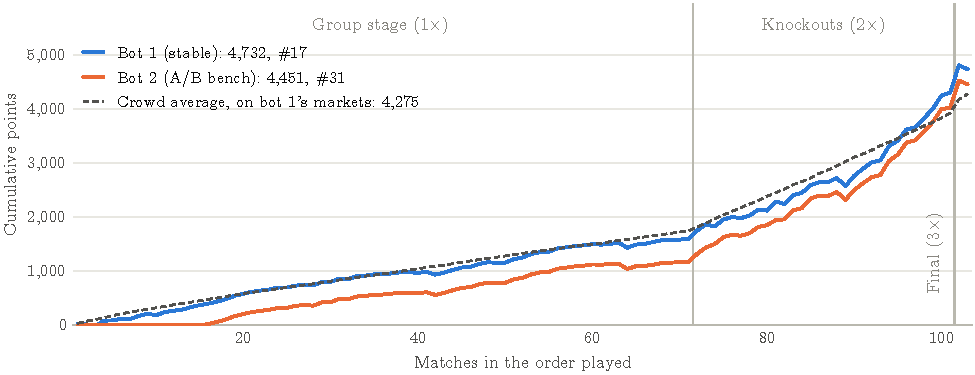
\includegraphics[width=\textwidth]{figures/cumulative_points.pdf}
\caption{Cumulative points over the \MatchesOne{} matches. The dashed line is the premium alone on
bot~1's markets: what submitting the crowd's average would have earned. Bot~2 earned nothing on
its first 15 matches (\cref{sec:incidents}).}
\label{fig:cumulative}
\end{figure}

\subsection{Where the edge came from}

The crowd's average forecast is biased upward: across bot~1's markets it averaged
\MeanCrowd\% against a realized rate of \BaseRate\%, while bot~1 averaged \MeanForecast\%.
\Cref{tab:categories} and \cref{fig:bias}a break this down. The crowd over-priced events most
on cards (\CrowdBiasCards{} points), player shots on target (\CrowdBiasPlayerSOT), penalties
(\CrowdBiasPenalties) and goal scorers (\CrowdBiasScorers). Bot~1 was much less biased on all of these except penalties, where both followed
similar base rates. Its edge per market was largest on timing windows (\EdgePerMarketTiming), cards
(\EdgePerMarketCards) and player shots on target (\EdgePerMarketPlayerSOT); on goal scorers the
smaller bias earned little (\EdgePerMarketScorers{} per market). On goals and results the crowd is nearly unbiased, because both follow the same
betting market; the edge there is modest per market (\EdgePerMarketGoals) but, over \MarketsGoals{} markets,
the largest in total. The losses are informative too: bot~1 under-predicted
team and total shots on target by \OurBiasAbsTeamSOT{} points on average (\EdgeTeamSOT{} edge), the leak that the total-SOT
scale of \cref{tab:constants} was introduced to close mid-tournament, and it also under-predicted
offsides and fouls.

\begin{table}[tbp]
\centering
\caption{Bot~1 by market type: points, edge over the crowd's average forecast, and bias (mean
forecast minus realized rate, in percentage points) for bot~1 and for the crowd's average.}
\label{tab:categories}
\begin{tabular}{@{}lrrrrrr@{}}
\toprule
 & & & & & \multicolumn{2}{c}{Bias (points)} \\
\cmidrule(l){6-7}
Market type & Markets & Points & Per market & Edge & Bot 1 & Crowd \\
\midrule
\inputtable{generated/tab_categories.tex}
\bottomrule
\end{tabular}
\end{table}

\begin{figure}[tbp]
\centering
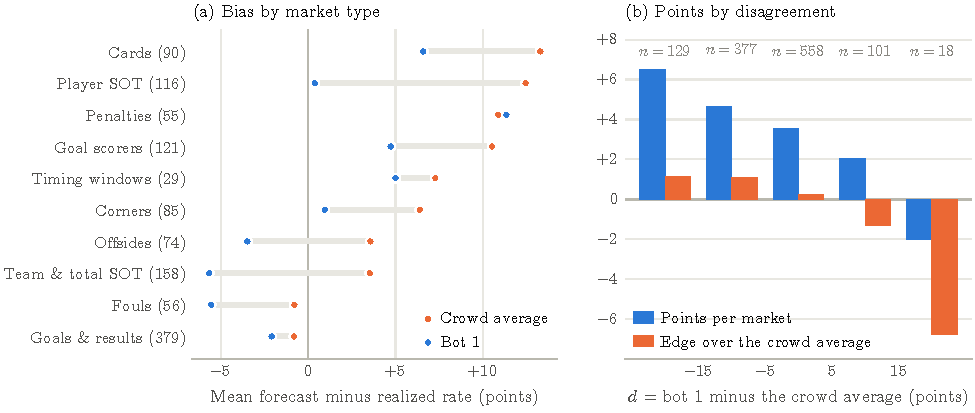
\includegraphics[width=\textwidth]{figures/bias_and_deviation.pdf}
\caption{(a) Bias by market type (types with at least 25 markets; SOT = shots on target): the
crowd's average over-prices most event types, bot~1 much less. (b) Points and edge per market
by how far bot~1 sat from the crowd's average.}
\label{fig:bias}
\end{figure}

\Cref{tab:deviation} and \cref{fig:bias}b group bot~1's markets by its disagreement with the
crowd, $d=100(p-\bar q)$. Points per market fall steadily from \DevPointsLowest{} when bot~1 sat more
than 15 points below the crowd to \DevPointsHighest{} when it sat 15 or more above. The edge column shows why:
pricing below the crowd beat the crowd's average forecast, pricing above it lost, consistent with
the crowd's upward bias. The premium is roughly constant across bins, so even forecasts within
five points of the crowd earned \DevPointsNear{} per market.

\begin{table}[tbp]
\centering
\caption{Bot~1 by disagreement with the crowd, $d$ = bot~1's probability minus the crowd's
average, in points. Mean forecasts and the realized rate are in percent; points, premium and
edge are per market.}
\label{tab:deviation}
\begin{tabular}{@{}lrrrrrrr@{}}
\toprule
Disagreement & Markets & Bot 1 & Crowd & Realized & Points & Premium & Edge \\
\midrule
\inputtable{generated/tab_deviation.tex}
\bottomrule
\end{tabular}
\end{table}

\subsection{Calibration}

In the club backtest the pricer tracks the diagonal within two percentage points in every bin
from 5\% to 95\% (\cref{fig:calibration}a), and it beat a constant 50\% forecast in all
\BacktestBeatHalf{} families and the historical base rate in \BacktestBeatBase{}
(\cref{tab:backtest}). In the tournament (\cref{fig:calibration}b) bot~1's expected calibration
error was \ECEOurs{} against \ECECrowd{} for the crowd's average. In the Murphy decomposition the
crowd's average is less reliable (\RELCrowd{} against \RELOurs{}) but slightly more resolved
(\RESCrowd{} against \RESOurs{}): it separates outcomes a little better while being shifted
upward. A share of the crowd's information is therefore not in the bots' inputs, which is an
argument for the researched inputs the agent supplied, and for more of them.

\begin{figure}[tbp]
\centering
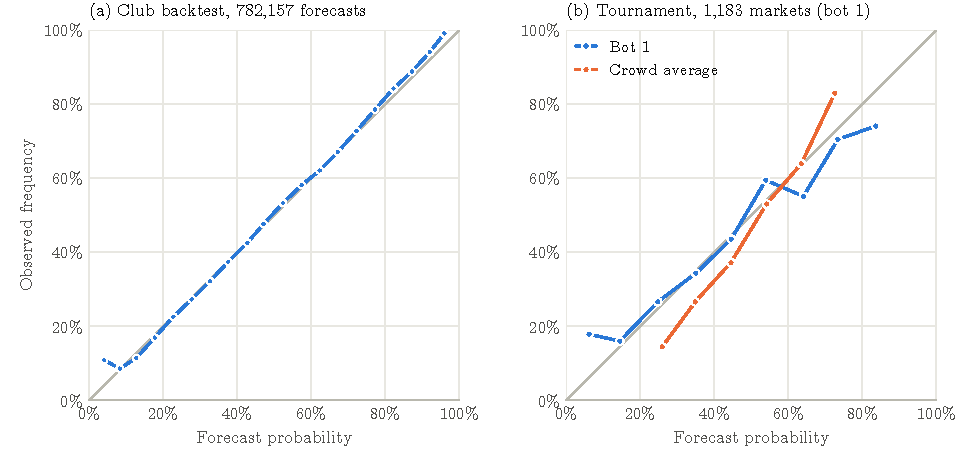
\includegraphics[width=\textwidth]{figures/calibration.pdf}
\caption{Reliability. (a) Walk-forward club backtest in 5-point bins. (b) The tournament in
10-point bins with at least 20 markets: bot~1 and the crowd's average forecast on the same
markets.}
\label{fig:calibration}
\end{figure}

\subsection{The A/B bench}

On the \CommonMarkets{} markets both bots played, their forecasts differed on
\DivergentMarkets{} markets in \DivergentMatches{} matches. Bot~2 was closer to the outcome on
\BotTwoBetter{} of them and bot~1 on \BotOneBetter{}, a net \ABNet{} points for bot~2 (95\%
interval \ABLo{} to \ABHi{}); over all common markets the mean Brier scores were
\CommonBrierOne{} and \CommonBrierTwo{}. The \GapPoints{}-point gap between the bots' totals is
entirely the \BotOneOnlyMarkets{} markets in the \BotOneOnlyMatches{} matches bot~2 missed
(\BotOneOnlyPoints{} points), less bot~2's gain on the divergent markets. The bench's
measurable contribution is therefore small. Its value was procedural: every change reached the
ranked entry through it, and it caught harmful ideas, such as the stronger count multipliers,
before they reached bot~1.

\subsection{Reproducing the final}

The archived code reprices the final's 20 markets offline from odds recovered from four goal
markets; 19 of the 20 forecasts equal what bot~1 submitted to the whole percent, and the
twentieth differs by one point (\code{probcup demo}). This is direct evidence that the archive
is the system that ran.

% ---------------------------------------------------------------------------
\section{Incidents and lessons}\label{sec:incidents}

\Cref{tab:incidents} lists the failures that changed the system. Most were operational rather
than statistical, and each left a rule behind.

\begin{table}[tbp]
\centering
\caption{Incidents and the rules they left.}
\label{tab:incidents}
\begin{tabularx}{\textwidth}{@{}l L L@{}}
\toprule
Date & What happened & Rule that stayed \\
\midrule
Jun 13 & The first scheduled run failed: commands register only at session start. & Scheduled prompts are self-contained (``read the playbook and execute it''). \\
Jun 16 & Bot~2 had been empty since launch while every pass reported it unchanged: the dual submission read bot~1's state. About 15 matches were lost. & Each bot is submitted its own values; every pass verifies both on the platform. \\
Jun 24 & A uniform low-event multiplier on every count statistic dropped bot~1 from about \#50 to \#94. & Per-statistic corrections, validated out of sample; never a uniform global dial. \\
Jun 26 & A stale ``benched'' override priced a starter at 5\% to register a shot on target. & Lineups are pulled automatically; inputs are scoped to one match; a staleness guard. \\
Jun 28 & Knockout boards re-phrased every question and the parser rejected them. & Phrasing normalization; new families built and tested the same day; a backlog scanner. \\
Jul 7 & A probe looked like a 10-of-13 winner, but the wins predated bot~1's last change. & Only settlements after the last change count toward promotion. \\
Jul 11 & A restart wiped the session's schedule; a morning run and a final pass never fired. & Two layers: session schedules run the researched passes; a durable job only raises alarms. \\
Jul 15 & A stale score-or-assist share on a prolific forward cost 94 points, the worst single market. & The score-or-assist consistency sweep on every board. \\
\bottomrule
\end{tabularx}
\end{table}

Three lessons generalize. \emph{Verify outcomes, not reports}: the costliest failure was silent,
because the submission summary was computed from the wrong state; only querying the platform
revealed it. \emph{Fail loudly rather than fall back}: when runs were missed, the tempting fix
was an automatic submission, but under relative scoring a careless forecast can lose points
while a skipped refresh loses only freshness, so the durable layer raises alarms and never
submits. \emph{Change the ranked entry only on large samples}: live samples were small and
correlated within matches, and three of four drift flags, as well as a promotion tally, turned
out to be noise once tested properly.

% ---------------------------------------------------------------------------
\section{Reproducibility}\label{sec:repro}

The repository is the archived system, restructured into an installable package with one
command-line entry point. Before anything moved, the code that ran the final (tag
\code{tournament-final}) was run against a fake outside world (stateful fakes of the
SportsPredict, ESPN, Polymarket and API-Football endpoints and a frozen clock) and every observable
effect was recorded: \BoardMarkets{} real markets priced for both bots, and thirteen command
scenarios down to each HTTP request, submitted value, printed line and file written. The
restructured code reproduces all of it exactly, and the suite runs offline in about 30 seconds
in continuous integration. The ten research studies and the full club backtest also produce
identical output before and after.

Every tournament result in this report (numbers, tables and figures) is generated from the
committed results export by \code{paper/build_assets.py}, and \code{make paper} rebuilds the
report from scratch; figures quoted from the research studies are in their committed outputs. The fitted
models and researched inputs as they stood for the final are committed; the raw event and club
data are downloaded by \code{probcup download-data}.

% ---------------------------------------------------------------------------
\section{Limitations}\label{sec:limitations}

The evidence comes from one tournament of \MatchesOne{} matches, and the edge over the crowd is
not statistically distinguishable from zero. We cannot compute counterfactual ranks, because
the distribution of leaderboard totals is not public, and the crowd's average is rounded to a
whole percent. The crowd data available \emph{during} the tournament were copied by hand from
16 matches; the full export only became available afterwards, so mid-tournament decisions rested
on far less evidence than this report. The quality of the agent's research inputs is not
measured separately from the models'. Finally, the archive deliberately keeps the defects that
ran live; the most consequential is that ``Will a substitute score or assist?'' was parsed as a
player named ``a substitute'' and priced at a generic prior, including in the final.

% ---------------------------------------------------------------------------
\section{Conclusion}\label{sec:conclusion}

Relative Brier scoring rewards two things: forecasting every market at least as well as the
crowd's average, which earns the field's dispersion, and beating that average where the crowd is
biased. A market-anchored engine delivers the first by construction; careful models of the
event types the crowd over-prices deliver the second, though over one tournament that edge is
small and uncertain. The larger lesson concerns operation. An agent can run a forecasting system
in production for weeks, but only inside rules that make its failures loud: verified submissions,
match-scoped inputs, alarms instead of fallbacks, and a separate entry for experiments.

\FloatBarrier
\section*{Acknowledgements and data}

Event data are from StatsBomb Open Data \citep{statsbomb}; club results and closing odds from
football-data.co.uk \citep{footballdata}; live odds from ESPN (DraftKings) and Polymarket; player
season rates from API-Football. This work is not affiliated with Jump Trading, SportsPredict or
FIFA.

\bibliographystyle{plainnat}
\bibliography{references}

% ---------------------------------------------------------------------------
\clearpage
\appendix
\section{Supplementary tables}\label{app:tables}

\noindent\begin{minipage}{\textwidth}\centering\small\captionsetup{hypcap=false}%
\renewcommand{\arraystretch}{1.0}
\captionof{table}{Walk-forward club backtest by question family: Brier score of the pricer, of a
constant 50\% and of the historical base rate, and the improvement over the base rate in Brier
points (hundredths). Each family has about \BacktestPerFamily{} forecasts.}
\label{tab:backtest}
\begin{tabular}{@{}lrrrr@{}}
\toprule
Family & Pricer & 50\% & Base rate & Gain \\
\midrule
\inputtable{generated/tab_backtest.tex}
\bottomrule
\end{tabular}
\end{minipage}

\vspace{12pt}
\noindent\begin{minipage}{\textwidth}\centering\small\captionsetup{hypcap=false}%
\renewcommand{\arraystretch}{1.0}
\captionof{table}{The \numfamilies{} question families and how many of the \BoardMarkets{}
archived questions each covers.}
\label{tab:families}
\footnotesize\setlength{\tabcolsep}{3pt}
\begin{tabular}{@{}lr@{\hspace{12pt}}lr@{\hspace{12pt}}lr@{}}
\toprule
Family & $n$ & Family & $n$ & Family & $n$ \\
\midrule
\inputtable{generated/tab_families.tex}
\bottomrule
\end{tabular}
\end{minipage}

\end{document}
